\documentclass[main.tex]{subfiles}
%% Current Author: PS
\setcounter{chapter}{7}
\begin{document}
\chapter{Atomic and Nuclear Processes}
\begin{content}
  \item the nucleus
  \item nuclear processes
  \item probability and radioactive decay
  \item fission and fusion
\end{content}
\section*{Candidates should be able to:}
\spec{understand the importance of the α-particle scattering experiment in determining the nuclear model}

In the famous scattering experiment an alpha source was placed in a lead container to produce a beam of alpha particles which were directed at a piece of gold leaf. Given the high energies of these alpha particles it was expected that they would simply crash through the gold leaf like a bullet through tissue paper. Instead, it was found that a few alpha particles were scattered through large angles and a small number came straight back.
\newpage
\begin{figure}[h]
  \begin{center}
    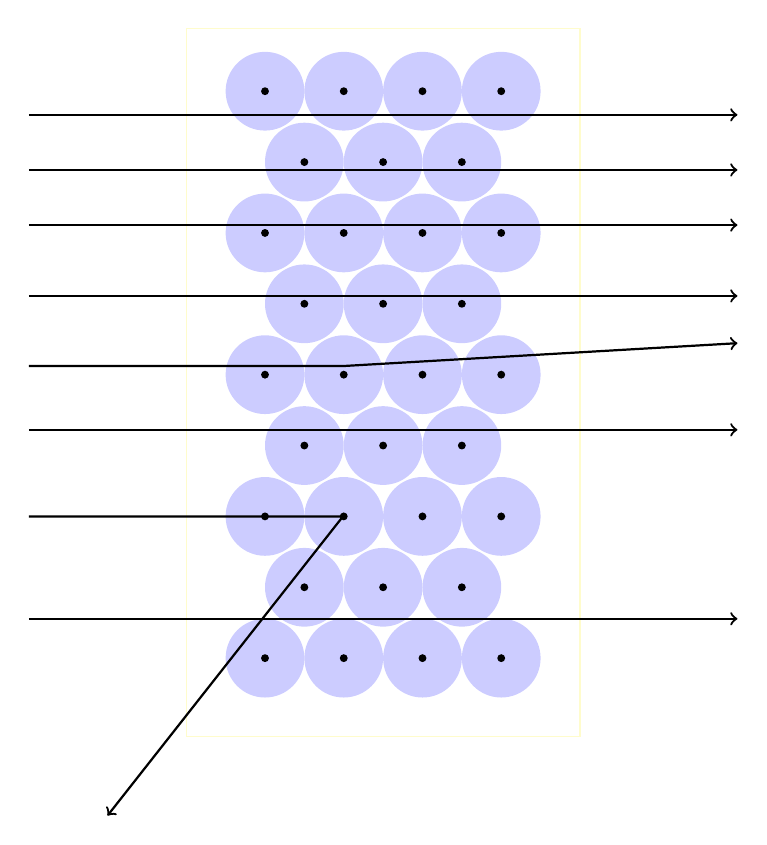
\begin{tikzpicture}
      \draw[yellow!20!white] (0,0) rectangle (5,9);
      \foreach \x in {1,2,3,4} {
        \foreach \y in {1,2.8,4.6,6.4,8.2} {
          \fill[blue!20!white] (\x,\y) circle (.5cm);
          \fill[black] (\x,\y) circle (0.05cm);
        }
      }
      \foreach \x in {1.5,2.5,3.5} {
        \foreach \y in {1.9,3.7,5.5,7.3} {
          \fill[blue!20!white] (\x,\y) circle (.5cm);
          \fill[black] (\x,\y) circle (0.05cm);
        }
      }
      \foreach \y in {1.5,5.6,3.9,6.5,7.2,7.9} {
        \draw[->, thick] (-2,\y) -- (7,\y);
      }
      \draw[->, thick] (-2, 4.71) -- (2,4.71) -- (7,5);
      \draw[->, thick] (-2,2.8) -- (1.99,2.8) -- (-1, -1);
    \end{tikzpicture}
  \end{center}
  \caption{Scattering of alpha particles by gold atoms}
  \label{fig:scattering}
\end{figure}

This occasional scattering implied that the gold nuclei are very small compared to the size of the gold atom and contain almost all of the atom's mass.

\spec{describe atomic structure using the nuclear model}

The nuclear model has a very small ($10^{-15}\ \si{\meter}$) nucleus which is positively charged and made up of protons and neutrons. Around this nucleus move the much lighter, negatively charged electrons.

\spec{show an awareness of the existence and main sources of background radiation}

The radiation referred to in this part of the specification is \emph{ionising} radiation. This is always present and is composed of both natural and artificial sources. The most common sources are shown in figure \ref{fig:rad-sources}.

\begin{figure}[h]
  \begin{center}
  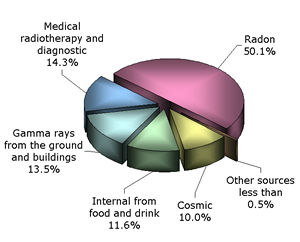
\includegraphics[width=0.8\textwidth]{figs/chapt-8/rad-sources.jpg}
\end{center}
  \caption{Background Radiation Sources in the UK (\url{http://www.npl.co.uk/educate-explore/factsheets/ionising-radiation/})}
  \label{fig:rad-sources}
\end{figure}

\spec{recognise nuclear radiations ($\alpha$, $\beta-$, $\gamma$) from their penetrating power and ionising ability, and recall the nature of these radiations}

\begin{table}[h]
\begin{tabular}{clll}
  \textbf{Radiation} & \textbf{Penetrating Power} & \textbf{Ionising Ability} & \textbf{Nature} \\
  $\alpha$ & low & high & helium-4 nucleus \\
  $\beta$ & medium & medium & electron \\
  $\gamma$ & high & low & electromagnetic wave \\
\end{tabular}
\caption{Three types of radiation}
\label{tbl:3-rad}
\end{table}

Table \ref{tbl:3-rad} shows the properties and nature of three types of radiation. Note that the penetrating power and ionising ability are inversely proportional as if a type of radiation is highly ionising it will interact with matter and therefore be stopped easily.

\newpage

\spec{write and interpret balanced nuclear transformation equations using standard notation}

In nuclear equations the individual species are written as $^A_Z X$ where $A$ is the \emph{nucleon} number, $Z$ is the \emph{proton} number and $X$ is the chemical symbol for the element. The three types of radiation are written as follows:
\begin{center}
  \begin{tabular}{llp{1cm}llp{1cm}ll}
    $\alpha$ & $^4_2 He$ & &
    $\beta$ & $^{0}_{-1} e$ & &
    $\gamma$ & $^0_0 \gamma$ \\
  \end{tabular}
\end{center}

The electron is given a `proton number' to enable the balancing of nuclear equations. In beta decay a neutron is transformed into a proton and an electron, therefore the nucleon number of the daughter does not change but the proton number increases by one. The beta particle's proton number of $-1$ balances this change.

In a balanced equation the sum of the proton numbers on each side must be equal, as must the sums of the nucleon numbers.

\begin{example}
  Write a balanced nuclear equation for the decay of carbon-14 by beta minus decay.

  \answer

  \begin{align*}
    ^{14}_6 C & \rightarrow  {}^{14}_7 N + ^{0}_{-1} e \\
    A: 14 &=  14 + 0 \\
    Z: 6 & =  7 - 1 \\
  \end{align*}
\end{example}

\spec{understand and use the terms nucleon number (mass number), proton number (atomic number), nuclide and isotope}

\begin{description}
  \item[Nucleon number] The total number of protons and neutrons in the nucleus.
  \item[Proton number] The number of protons in the nucleus.
  \item[Nuclide] A specific number of protons and neutrons which makes a unique nucleus. Usually defined by a combination of proton number / element name and mass number. E.g. carbon-14, $^{14}_6 C$.
  \item[Isotope] Isotopes are nuclei of the same element with different mass numbers, i.e. the same number of protons but different numbers of neutrons.
\end{description}

\spec{appreciate the spontaneous and random nature of nuclear decay}

Radionuclei decay spontaneously and randomly because of the fundamentally quantum nature of the process. This means that while one can make predictions about a collection of nuclei using half-life it is impossible to predict when any particular nucleus will decay.

\spec{define and use the concept of activity as the number of decays occurring per unit time}

Activity is defined in this way, but measured by counting the number of ionisation events occurring in a detector per unit time.

\spec{understand qualitatively how a constant decay probability leads to the shape of a radioactive decay curve}

A constant probability of decay means that the total rate of decay of a sample is proportional to the number of nuclei remaining. This means that the number of nuclei remaining decreases with decreasing rate. The activity is proportional to the number of nuclei remaining so it also decreases with decreasing rate.

\spec{determine the number of nuclei remaining or the activity of a source after a time which is an integer number of half-lives}

One half-life is the time taken for half of a sample to decay. Therefore after three half-lives the amount remaining is $\left(\frac{1}{2}\right)^3 N_0$ where $N_0$ is the original amount.

\spec{understand the terms thermonuclear fusion, induced fission and chain reaction}

\begin{description}
  \item[Thermonuclear fusion] This is the combining of two nuclei to form a new, heavier nucleus. It is the type of nuclear reaction which occurs in stars where hydrogen nuclei fuse to form helium. The electrostatic repulsion between the nuclei is overcome by the thermal energy of the particles involved,  meaning that thermonuclear fusion can only occur at extremely high temperatures.
  \item[Induced fission] This is the splitting of a large nucleus into two smaller, daughter nuclei. This does not occur spontaneously but must be induced by the collision of a neutron with the nucleus.
  \newpage
  \item[Chain reaction] When a neutron induces fission in a large nucleus it is usually the case that as well as the two daughter nuclei, several further neutrons are released. These neutrons can then go on to cause further induced fission events in other heavy nuclei. This is known as a chain reaction.
\end{description}
\end{document}
